\section{Branch and Bound Approach}
\label{cha:branchandbound}

This chapter is motivated by the fact that branch and bound search is
one of the most widely used tool for solving large scale NP--hard
optimization problem. This technique has gained tremendous success in
some domain specific areas, such as Boolean satisfiability test (SAT)
and mixed integer programming (MIP). In the SAT community, improved
versions of the Davis-Putnam-Logemann-Loveland (DPLL) algorithm are
able to effectively solve problems with millions of variables and
constraints \cite{harmelen}.

%=================================================
\subsection{Foundation of Branch and Bound Search Approach}
\label{sec:bnb.idea}

This section shows how to formulate the 0--1 loss problem such, that
it is possible to apply the branch and bound search
strategy. Following from the definition of the 0--1 loss optimization
problem given in Chapter \ref{cha:background}, the 0--1 loss function
can be written as
$$L(\w) = \sum_{i=1}^N \mathbb{I} [t_i \w^T \xi \leq 0] = \sum_{i=1}^N l_i,$$ 
where $l_i =\mathbb{I} [t_i \w^T \xi \leq 0]$ denotes the individual 0--1 loss of point $\xi$. We have
\[ \begin{split}
l_i = 0 &\Leftrightarrow t_i \w^T \xi > 0 \\
l_i = 1 &\Leftrightarrow t_i \w^T \xi \leq 0. \\
\end{split} \] 
Furthermore, let $\l=(l_1, l_2, \dots, l_N)$ be the loss vector
consisting of all individual losses. It can be seen that a specific
assignment of the loss vector corresponds to a system of linear
inequalities. For example, the loss vector $\l=(0,1,0)$ for a training
dataset of $N=3$ points corresponds to
$$
\left\{
     \begin{array}{l}
       t_1 \w^T \x_1 > 0\\
       t_2 \w^T \x_2 \leq 0\\
       t_3 \w^T \x_3 > 0
     \end{array}
\right.
$$ where $t_1, t_2, t_3, \x_1, \x_2, \x_3$ are constants given by the
training dataset, so the above is a system of linear inequalities.

Let $\S_{\l}$ denote the system of linear inequalities induced by the
loss vector $\l$.  $\S_{\l}$ can be solved quite efficiently using the
well studied linear programming (LP) technique, e.g., by using a LP
solver like that by \cite{lpsolve}. There is, however, a subtlety here
that needs to be addressed. One can see that if $\w'$ is a solution of
$\S_{\l}$, then for any real constant $c > 0$, $c \w'$ is also a
solution. Therefore, if $\S_{\l}$ is consistent, it will have
infinitely many solutions. In this case, a LP solver will return a
message saying that the solution set is infinite. One trick can be
used here is to specify that the bias, $w_0$, must be either $1$ or
$-1$, because these are the only two possible values for the bias when
$\w$ is scaled by $c=1 / |w_0|$. Here it is assumed that $w_0 \not=
0$, which is reasonable, because otherwise the decision hyperplane
``must'' go through the origin, which is rare in practice. So, a
specific solution of $\S_{\l}$ is obtained by using LP solver to solve
for $\{ \S_{\l} \land (w_0=1) \}$ or $\{ \S_{\l} \land (w_0=-1) \}$,
whichever has solution. If both these are inconsistent, then $\S_{\l}$
is also inconsistent.

To sum up, a loss vector $\l$ induces a system of linear inequalities,
for which a LP solver can either gives a concrete solution $\w'$ if
the system is consistent (in this case we call the loss vector
\emph{feasible}), or give no solution if the system is inconsistent
(in this case we call the loss vector \emph{infeasible}). Thus, the
0--1 loss optimization problem is now equivalent to finding a feasible
loss vectors $\l^*$ with minimal sum of its components (which is the
sum of 0--1 losses):
$$\l^* = \text{arg min}_{\l : \text{ feasible}} \sum_{i=1}^N l_i.$$
The optimal weight vector, $\w^*$, is then the solution of the system
of inequalities induced by $\l^*$ ($\S_{\l^*}$), which can be easily
obtained using a LP solver as discussed.

Clearly, a branch and bound algorithm may be used to find $\l^*$,
where in each step we branch on the first unassigned component of the
loss vector, $l_i$, for two possible subsets corresponding to $l_i =
0$ or $l_i = 1$. The basic algorithm is detailed in the next section,
with more advanced algorithms follow in the section after that.

%=================================================

A step by step explanation are being provided next for the purpose of an implementation (if needed).

\begin{figure}
\caption{
Final BnB Algorithm Combining All Heuristics. \\
\text{\hspace{2.15cm}} $Input$: Dataset of training data points $ \boldsymbol{X}$, their labelled targets $\t$. \\
\text{\hspace{2.15cm}} $Output$: Optimal weight vector $\w^*$ minimizing 0--1 loss.
}
\label{alg:BnB.Final}
\begin{algorithmic}[1]
\Function{Find-Optimal-01Loss-Solution-Final}{$\X, \t$}
\State $\tilde{\w} \gets $ approximated weight vector given by a fast classifier
\State $\tilde{\l} \gets $ loss vector implied by $\tilde{\w}$
\State $\w^* \gets \tilde{\w}$
\State $loss_{min} \gets \sum_{i=1}^N \tilde{l}_i$ \Comment{Set initial bound to $L(\tilde{\w})$}
\State $\l_\emptyset \gets $ loss vector with all components unassigned
\State \Call{Branch-and-Bound}{$\l_\emptyset, 0$}
\State \Return $\w^*$
\Statex
\Procedure{Branch-and-Bound}{$\l, loss$}
   \If {(all components of $\l$ are assigned)}
      \State $\w^* \gets$ a specific solution of $\S_{\l}$ \Comment{update optimal solution}
      \State $loss_{min} \gets loss$
   \Else
      \State Find index $i$ of the unassigned component of $\l$ with greatest $|\tilde{\w}^Tx_i|$
      \State $\l' \gets$ \Call{Propagate-Loss}{$\l, i, \tilde{l}_i$}
      \If {$sum(\l') < loss_{min}$}
         \State \Call{Branch-and-Bound}{$\l'$}
      \EndIf
      \State $\l' \gets$ \Call{Propagate-Loss}{$\l, i, 1 - \tilde{l}_i$}
      \If {$sum(\l') < loss_{min}$}
         \State \Call{Branch-and-Bound}{$\l'$}
      \EndIf
   \EndIf
\EndProcedure
\Statex
\Function{Propagate-Loss}{$\l, i, lossValue$} \Return {new loss vector $\l'$}
   \State $\l' \gets \l$
   \State $l_i' \gets lossValue$   
   \State $\t' \gets $ targets prediction vector implied by $\l'$ 
   \State Let $\Phi =$ convex hull created by $\{ \boldsymbol{x_k} \; | \; t_k'=t_i' \}$ 
   \If {$\exists \boldsymbol{x_j} \in \Phi$ such that $l_j$ is assigned AND $t_j' = -t_j'$}
      \State $l_i' \gets +\infty$ \Comment{convex hulls intersect $\rightarrow$  infeasible}
   \Else
   \For{p:=1 \text{ {\bf to} } N}
      \If{$\boldsymbol{x_p} \in \Phi$ AND $l_p$ unassigned}
         \State $t_p' \gets t_i'$ \Comment{propagate loss to unassigned points inside $\Phi$}
         \State $l_p' \gets \mathbb{I} [t_p' \not= t_p]$
      \EndIf
   \EndFor
   \EndIf  
   \State \Return $\l'$
\EndFunction
\Statex
\EndFunction
\end{algorithmic}
\end{figure}

 
Empirical tests (see Figure \ref{fig:BnBtimes}) shows that for bigger
problem ($N>40$), Algorithm \ref{alg:BnB.Heuristics} with the loss
propagation heuristic outperforms all other algorithms in this
chapter. It is, however, slower for smaller problem. This is expected
as with increasing size, the (high) cost to calculate loss propagation
starts to pay off.



%=================================================
\subsection{Techniques for Branch and Bound Improvement}
\label{sec:bnb.improvement}

It was discussed in the previous section, that for the branch and
bound (BnB) approach to be practically useful, further improvement is
required. Heuristics are well known to be effective mean for this
purpose, as detailed in Chapter 3 of \cite{russell}. Thus, this
section proposes several heuristics that improve the performance of
the basic branch and bound algorithm as detailed in the following
three subsections.

%===========================
\subsubsection{Initial Bound Approximation}
\label{sec:bnb.ordering}

The first and simplest technique for performance improvement is to set
the initial value of $loss_{min}$ to some initial approximation of the
optimal loss value. For example, one can use some fast classifier to
approximate the optimal decision hyperplane, then calculate the
corresponding 0--1 loss value, and initialize $loss_{min}$ to that
value as an initial bound. This technique is rather simple, but quite
effective. Basically, all search paths with loss value greater or
equal to the value of the initial bound are pruned. For example, if
there are 20 points in the training dataset, the number of all
possible search paths is $2^{20} \approx 10^6$, if the initial bound
is set to 5, the number of search paths to be considered is only ${20
  \choose 5} \approx 10^4$, which corresponds to a 100 times reduction
in the size of the search space. \footnote{Technically, the reduction
  is less, because even without an initial approximated bound, the
  bounding condition at step 19 of Algorithm \ref{alg:BnB.Basic} would
  still reduce the size of the search tree significantly.} The
implementation of this technique is also quite simple and it is
included in Algorithm \ref{alg:BnB.BestFirst} at step 5, where the
initial bound is set to the loss value induced by the approximated
separation hyperplane.

%===========================
\subsubsection{Best-First Search}
\label{sec:bnb.ordering}

First, let's have a look at an example illustrating the importance of
the order, in which components of $\l$ are assigned. For a fictional
problem of 40 data points with optimal 0--1 loss = 1, and a fixed
assignment order from the first to the last point, if in the optimal
solution, the first point is misclassified, then in Algorithm
\ref{alg:BnB.Basic}, the loss value of the first component, $l_1$,
must be assigned to 1, which would be done only after all combinations
where component $l_1$ is $0$ have been checked, which costs
$O(2^{39})$, an infeasible number. Clearly, for this example to be
feasible, the resolution is to either have $l_1$ assigned correctly to
1 from the beginning, or change the assignment order such, that $l_1$
is assigned lastly. The strategy discussed in this subsection takes
into account both these resolutions.

It was suggested in the previous subsection, that a fast classifier,
e.g., logistic regression or linear SVM -- both are $O(N)$, could be
used to approximate the optimal decision hyperplane, and then used to
approximate the initial bound. It turns out that having an
approximated decision hyperplane would also help to determine the
assignment order and the assignment value as illustrated in Figure
\ref{fig:svm_hyperplane}. Under the assumption that the optimal
decision hyperplane is not very far from the approximated hyperplane,
clearly, the loss values of points that lies closer to the
approximated hyperplane, like point $C$ in the figure, are more likely
to be changed comparing to points lying far away, like points $A, B$
in the figure. This fact can be exploited to design a best-first
search strategy as follows. The loss values of points farther away
from the approximated decision hyperplane are assigned first, and they
are assigned to the same loss values as indicated by the approximated
decision hyperplane. For example, considering only three points $A, B,
C$ in Figure \ref{fig:svm_hyperplane}, the loss value of $B$ would be
assigned to 0 first, then the loss value of $A$ assigned to 1, then
the loss value of $C$ assigned to 0, then after some branching and
bounding, the loss value of $C$ will be changed to 1 in the optimal
solution, but the loss values of $A$ and $B$ remain the same.

The above strategy allows to find the optimal solution in a very early
stage of the search process. This has twofold benefits. First, it
increases the effectiveness of the bounding condition
dramatically. Second, if the algorithm reaches time limit and needs to
exit, there is a high probability that the current solution is the
optimal one, or close to it, and it is guaranteed to be no worse than
that of the initial approximation (e.g. given by SVM or some other
classifier). As such, it is an $anytime$ algorithm. The algorithm for
this best-first search strategy is listed in Algorithm
\ref{alg:BnB.BestFirst} with detailed description given in the next
paragraph. It is important to mention here, that the distance of point
$\xi$ to the decision hyperplane defined by $\w$ is directly
proportional to the absolute value of their dot product, $| \xi \cdot
\w |$, as detailed in subsection 4.1.1 of \cite{bishop06}, hence the
assignment in decreasing order of the distance from given points to
the decision hyperplane defined by $\w$ is equivalent to the
assignment in decreasing order of the absolute value of their dot
product with $\w$. Practical tests on problems of size $N=50$ using
the SVM as an initial approximation shows that the time for Algorithm
\ref{alg:BnB.BestFirst} to reach the optimal solution in the search
tree is on average under 3 seconds. However, it takes much longer to
finish the whole search.

\begin{figure}[here]
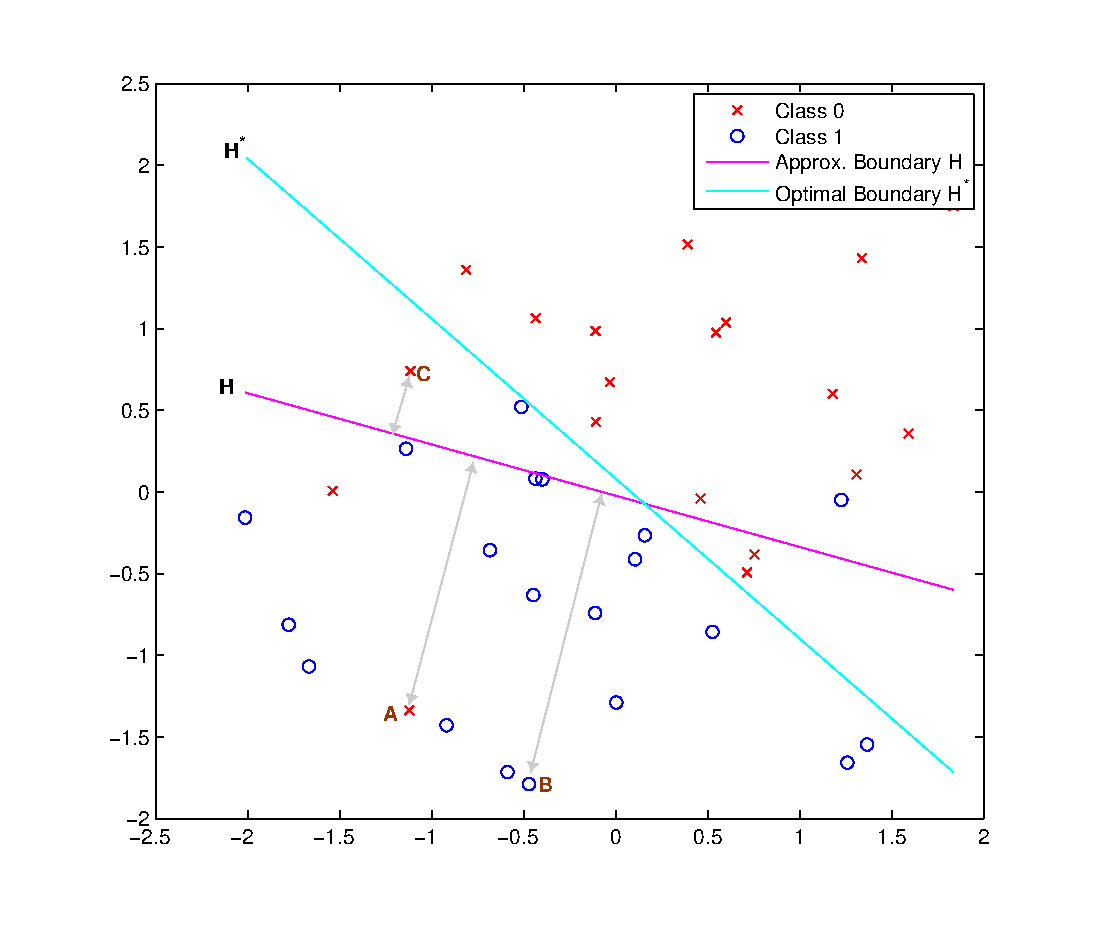
\includegraphics[width=0.50\textwidth]{images/fig31_svmhyperplane.eps}
\caption{ The use of an initial decision hyperplane to direct the loss
  vector's assignment order and value.  This plot shows an initial
  approximated decision hyperplane, $H$, given by the SVM method, with
  0--1 loss = 7, the optimal hyperplane, $H^*$, has 0--1 loss =
  4. Data point $A$ is misclassified by $H$, hence would have loss
  value = 1. Data point $B$ is correctly classified, hence would have
  loss value = 0. Because $A$ and $B$ lie far from $H$, their loss
  value remains the same when classified by the optimal decision
  hyperplane $H^*$, which is assumed to not have much deviation from
  $H$. On the other hand, because point $C$ lies much closer to $H$,
  its loss value changes when classified by $H^*$. Thus, a good
  assignment strategy is to assign in order from points farther away
  to points closer to $H$, and assign the same loss value as
  classified by $H$ first.  }
\label{fig:svm_hyperplane}
\end{figure}


%===========================
\subsubsection{Loss Propagation}
\label{sec:bnb.heuristic}

This subsection studies the idea of using the convex hull created by
data points of a same class to develop a heuristic, which we term
\emph{loss propagation}, to improve performance of branch and bound
search for 0--1 loss. As shall be seen, loss propagation turns out to
be quite powerful as it legitimately enforces some unassigned
components of the loss vector to have a specific value, which
significantly reduce the search tree and automatically ensures
feasibility of the loss vector.

\begin{figure}[here]
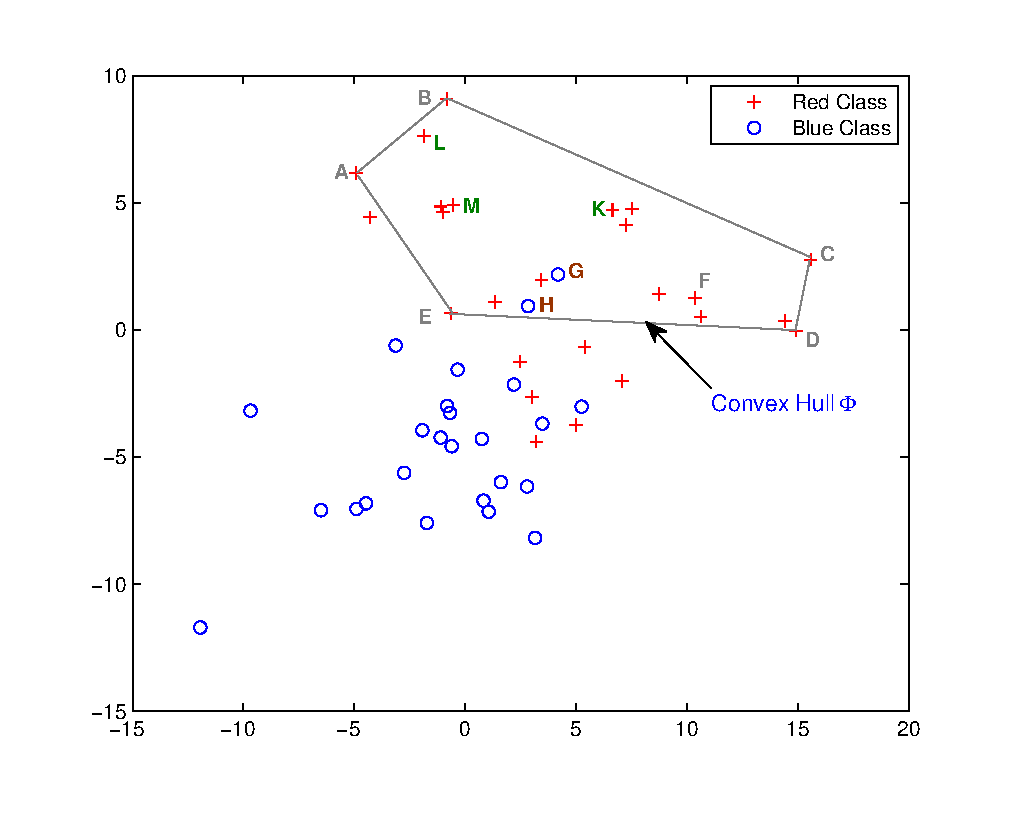
\includegraphics[width=0.50\textwidth]{images/fig32_convexhull.eps}
\caption{ This plot shows that the convex hull created by points,
  whose loss value has already been assigned, can provide an
  admissible heuristic and additional pruning.  In this plot, it is
  assumed, that in the current search path, points $A, B, \dots F$
  have loss value assigned to 0, which implies that they are
  (correctly classified) in the red class, all other points are
  unassigned. The convex hull $\Phi$ created by points $A$ through $F$
  is a convex polygon in this 2D example, and every point inside it
  must be assigned to the red class in order for the assignment of the
  loss vector to be feasible. Thus, for example, point $G, H$ must
  have loss value = 1 (to be misclassified as red class), implying an
  admissible heuristic value = 2, points $K, M, L$ and all other red
  points inside $\Phi$ must have loss value = 0 (correctly classified
  as in red class), hence they require no further branching.  }
\label{fig:convexhull}
\end{figure} 


In Figure \ref{fig:convexhull}, for simplicity it is assumed, that the
loss values of data points would be assigned in alphabetical order,
i.e., $A, B, \dots, L, \dots $, and in the current search path, loss
values of points $A$ through $F$ have been assigned to 0, and loss
values of all other points are unassigned. Clearly, points $A$ through
$F$ are correctly classified (because their loss is 0), hence they all
belong to their true class -- the red class. The convex hull, $\Phi$,
of points $A$ through $F$, in this 2--D example, is a convex polygon
drawn in grey in the figure. Now, let's consider point $G$, which lies
inside the convex polygon $\Phi$. If its loss value is assigned to 0,
meaning it is correctly classified as in the blue class, then the set
of inequalities induced by the current path is infeasible, because
there is no possible decision hyperplane that can separate point $G$
from points $A$ through $F$. Therefore, point $G$ must be
misclassified with loss value = 1. Similarly, point $H$ must also have
loss value = 1. On the other hand, if point $K$ is misclassified to
the blue class, then, again, there's no possible decision hyperplane
that can separate it from points $A$ through $F$. Therefore, point $K$
must belong to the red class, and so have loss value = 0. The
conclusion is that all points inside the convex hull created by points
of a given class must be assigned to that class in order for the
assignment to be feasible. Specifically, in Figure
\ref{fig:convexhull}, the loss value of all red points inside $\Phi$,
such as $K,M,L$, must be 0, the loss value of all blue points, such as
$G, H$ must be 1. So we have an admissible heuristic of loss = 2, and
forced the loss value of 15 points inside $\Phi$ to be assigned
without branching, which is a significant reduction in size of the
search tree.

Another observation is that if, for example, in Figure
\ref{fig:convexhull}, in the current search path, points $A$ through
$F$ are assigned to the red class, and point $H$ with some (any) other
points outside of $\Phi$ are assigned to the blue class, then we can
decide that the current loss vector is infeasible, because the two
convex hulls created by points of the same class intersect with each
other, hence there is no possible decision hyperplane that can
separate these two classes. Therefore, in order for the loss vector to
be always feasible, we can not assign the loss value of one point, if
such assignment makes the two convex hull corresponding to each class
intersect with each other.

The remaining problem to be addressed is how to test if a point
$\boldsymbol{p} \in \R^D$ is an interior point of the convex hull
created by some other points $\boldsymbol{p_1, p_2, \dots, p_k} \in
\R^D$. If points are in $\R^2$, this can be done efficiently in $O(n
\log n)$ time, e.g., by determining edges of the convex hull as
detailed in Section 33.3 of \cite{cormen}, and then test if the given
point is in the correct side of each edge. However, it is not known if
any efficient algorithm to determine edges of convex hull in $\R^D$
exists. Thus, we have to approach this problem from another direction
using the Barycentric coordinate system, which says point
$\boldsymbol{p}$ is an interior point of the convex hull created by
points $\boldsymbol{p_1, p_2, \dots, p_k}$ if the homogeneous
barycentric coordinates of $\boldsymbol{p}$ with respect to
$\boldsymbol{p_1, p_2, \dots, p_k}$ is all non-negative. This is
equivalent to solving the following linear programming
problem \footnote{This solution was suggested to me by Stephen Gould,
  CECS, Australian National University.}: find $\boldsymbol{u}$ such
that
$$
u_i \geq 0 \text{ for } i = 1,2, \dots, k \quad \quad \land \quad \quad
\sum_{i=1}^k u_i = 1 \quad \quad \land \quad \quad
\sum_{i=1}^k u_i \boldsymbol{p_i} = \boldsymbol{p}. 
$$ If such $\boldsymbol{u}$ exists, then point $\boldsymbol{p}$ lies
in the convex hull of points $\boldsymbol{p_1, p_2, \dots, p_k}$,
otherwise it does not.

To sum up, the above analysis of the convex hull created by the loss
assignment identified three possible improvements for the branch and
bound search of 0--1 loss.
\begin{enumerate}
\setlength{\itemsep}{0pt}
\setlength{\parskip}{0pt}
\item All points inside the convex hull of assigned points of one
  class must be forced to that class.
\item The sum of forced and assigned components of the loss vector is
  a lower bound.
\item If the convex hull of assigned points of one class intersects
  with that of other class, the current loss vector is infeasible,
  because no hyperplane can separate the two intersecting convex
  hulls. Thus, loss value assignment to any point must not make these
  two convex hulls intersect.
\end{enumerate}
All these points are accounted in Algorithm \ref{alg:BnB.Heuristics},
where the high level concept should be apparent.


%=================================================
\subsection{Evaluation of the Branch and Bound Approach}
\label{sec:bnb.final}

In the following subsections, we propose a final branch and bound
algorithm that combines all discussed heuristics and analyze its
running time.

%======================
\subsubsection{Combination of Heuristics}

The previous section discussed three strategies to improve the
performance of the basic algorithm (Algorithm
\ref{alg:BnB.Basic}). Actual implementation and tests (see Figure
\ref{fig:BnBtimes}) concludes, that the best algorithm is the one that
combines all these strategies. This is an expected result, as the
strengths of each strategy would complement each other in a combined
algorithm. This combined algorithm is detailed in Algorithm
\ref{alg:BnB.Final}.

\begin{figure}[here]
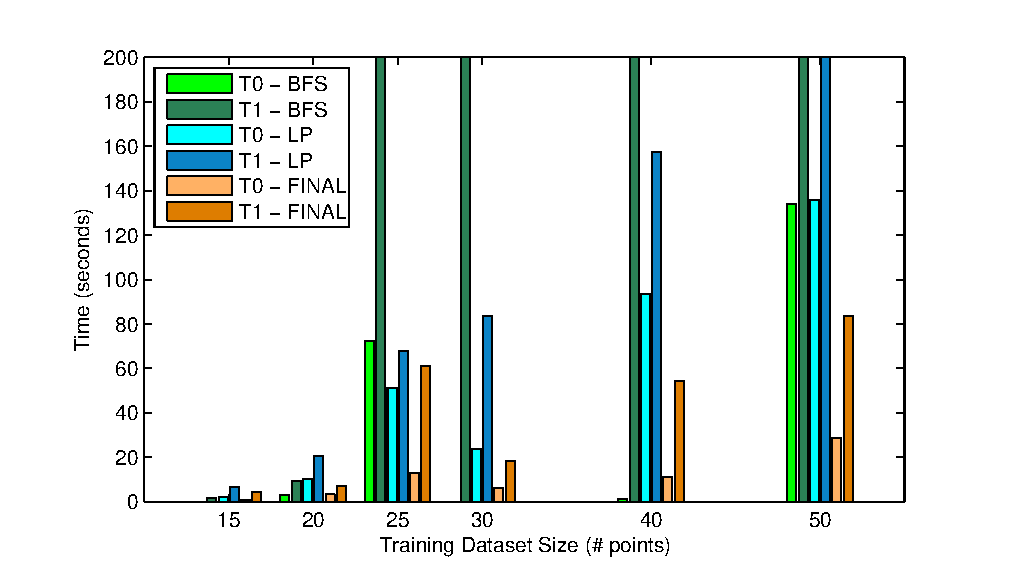
\includegraphics[width=0.50\textwidth]{images/fig33_BnBtimes.eps}
\caption{ This plot compares the time to reach the optimal solution
  (T0) and the total running time (T1) of best first search algorithm
  (BFS), loss propagation algorithm (LP), and the final algorithm
  (FINAL), which combines both BFS and LP. A running time limit of 200
  seconds is set for all algorithms. Clearly, BFS reaches the optimal
  solution early, but takes a long time to finish exploring the whole
  search space. LP, on the other hand, reaches the optimal solution
  much slower, and thank to the high cost of calculating the LP
  heuristic, it also runs slower than BFS for smaller problems, but it
  pays off very quickly when $N$ increases, hence outperforms BFS
  significantly for $N>25$. The combined algorithm, FINAL, has the
  strengths of both BFS and LP as it reaches the optimal solution
  early, and prunes the search space effectively using the loss
  propagation. Thus, it is the best among these algorithms.}
\label{fig:BnBtimes}
\end{figure} 

